\begin{savequote}[75mm] 
If I have seen further it is by standing on the shoulders of giants
\qauthor{Isaac Newton} 
\end{savequote}

\chapter{Introduction}

\newthought{Bioinformatics is in its very nature multi--disciplinary}: biotechnology methods are used to capture the data, mathematical and statistical models are necessary to make sense of it; and software/hardware it is necessary to process all the information and everything should be seen under the prisma of the existing biological knowledge.

Techniques and methods trying to uncover the logic behind cellular proceses are in constant development. The success of such methods is usually related to the ability of isolating a particular state/measurement of the organic material (e.g. level of expression of a single protein, number of mutations of a gene in a population, etc.). However,  cellular functions of a higher level and organism's processes can only be study with a more holistic approach.

Integrating information from different experiments in context with the current knowledge-base is one of the most recurrent duties that researchers have to accomplish, this task however takes another dimension when the goal is aimed to a generic scope, and the strategy to connect related data sets should work in similar scenarios.

The challenges of integrate data in a more generic scope go from technical (e.g. incompatibilities of the storage systems) to structural (e.g. two datasets can refer to the same entity using different identifiers), but in overall the major challenge is to not lose the meaning on the connection (e.g. linking proteins and genes and knowing what is their relationship).

Integration of data usually refers to connecting data in low level, by means of storing aggregated information from several sources or by saving links to where the source is. However it is also possible to integrate on a higher level, where information is not saved and the aggregates are built on the fly and visualised in order to provide a wider view.

This project explores both, Integration and visualisation of information in bioinformatics; the rest of this introduction presents the state of the art and base technologies in both fields. Chapter 2 presents the efforts executed during this doctorate that contribute to the ways data is integrated in bioinformatics projects. Chapter 3 describes our inputs to the visualisation of data in bioinformatic, focusing in particular in a web tool for the visualisation of protein-protein interactions. The final chapter contains the conclusions of the project.


\section{Integration of information}
\subsection{State of the art}
The latest version of the Nucleic Acids Research Database Issue added another 58 databases to the online collection hold by the journal, which then reached the number of 1552 databases \cite{FER2014}. This collection is far from including every single database, but it is  a good reflection of the amount of available resources.
The approaches to integrate data from all those sources are themselves heterogenous and they focused on different types of integration, from simply linking resources; to development of complex structures of aggregated information. In \cite{GOB2008} the authors categorise the different techniques used to integrate data in bioinformatics into 8 approaches, and then this categories were reorganised in \cite{ZHA2011b} into:
\begin{description}
\item[Data warehousing:] 			A centralised repository were the information from different sources is copied and processed to be kept  in a single place. providing a single access point to their data. However the preprocessing of the data is usually a complex process and the posterior additions or editions might require a lot of work.
\item[Federated databasing:] 		Multiple sources agree to follow a similar structure in order to allow a standard query over several instances. By dealing with smaller datasets than the data warehousing approach the complexity of post-processing is simplified, however it requires that the providers deal with the extra work of maintaining their data as the federated database agreement stablishes.
\item[Service oriente integration:] 	Definition of a protocol for requests and responses to obtain data or execute services. The 2 standards widely used are SOAP (Simple Object Access Protocol) services and REST (REpresentational State Transfer) services, where the latter is getting momentum because of its simplicity. However this also requires big commitment from providers about creating and maintaining the services, and also increasing and maintaining the specifications for the different domains.
\item[Semantic integration:] 		Structures the data using semantic web standards(e.g. RDF, OWL) in order to make it ``machine-readable'' and be able to deduce meaningful associations. The conversion of the data into RDF files might not be a trivial work, and it has similar problems to the one mentioned above because it maintains copies of the information in a separate format. 
\item[Wiki-based integration:] 		Cooperative effort where the community inputs information in a open and unstructured way, which can reach a highly reliable status as has been shown by the wikipedia case, but is completely dependent on the adoption of the community, and also given the unstructured nature of the data is hard to manipulate for automatic analysis.
\end{description}

We now present some of the most representative projects that have attempted to integrate data and offer a solution for this need in the bioinformatics field, by using one or more of the mentioned approaches. 

\subsubsection{Sequence Retrieval System}
The Sequence Retrieval System, better known in bioinformatics as SRS, was probably the most successful project before the introduction of Next Generation Sequencing (NGS) technologies, originally aimed at facilitating access to biological sequences databases \cite{ETZ1996}, it grew to became an integration system of both data retrieval and applications fro data analysis.

SRS was developed following an object-oriented design with the strategy of taking advantage of raw text files, that were the \emph{de-facto} standard on molecular biology analysis. By dealing only with text files, SRS was getting faster retrieving speed and saving storage space, mainly because data was neither store nor parsed, only indexed \cite{ZDO2002}.

The obtained indexes were there linked via meta-data, offering the user access to the original source plus links to any conceptually related database; all of it presented on a web-based interface, the automatically created interface for different sources and applications can be complicated for beginners, however SRS provide ways to create customised interfaces.

Probably the most important instance of SRS was the one installed at the European Bioinformatics Institute (EBI), which used to give access to the major databases produced and maintained at the EBI. However by December 2013 the service was decommissioned as the service was considered redundant with the efforts to maintain multiple web services. Currently SRS technology is now property of Instem\textsuperscript{TM} and a list of available servers can be seen at http://bioblog.instem.com/download/srs-parser-and-software-downloads/public-srs-installations/


%\section{Current Projects for Data Integration in Bioinformatics}
\subsubsection{BioWarehouse}
BioWarehouse is an open source toolkit to create data warehouses using MySQL or Oracle \cite{LEE2006}. The motivation behind this project is to provide  a single access point that supports Standard Query Language (SQL) running on a high performance environment.
This projects follows the data warehousing approach to integrate data, however the authors argue that it can be use as a part on a federated system and therefore, it doesn't aim to replace existing distributed system but o to complement them.

The development efforts were focused on the creation of a relational data model that supports the information from several biologic entities. Figure ~\ref{fig:biowarehouse} shows the main datatypes that are defined in the BioWarehouse scheme including, Taxon, BioSource, Nucleic Acid, Gene, Protein, Feature, Reaction, Chemical and Pathway. It was the objective of the creators that such model evolves including other entities, but at the same time keeping the model as simple as possible.

\begin{figure}  
\centering
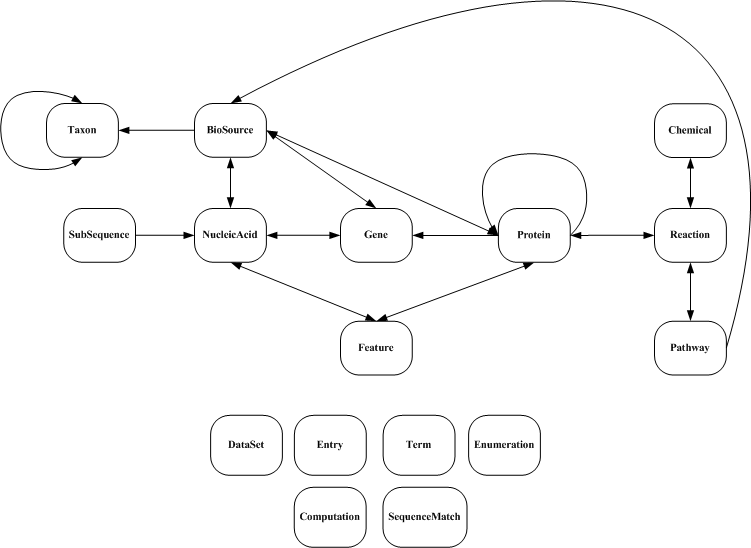
\includegraphics[width=4in]{figures/biowarehouse.png}
\caption[Original BioWarehouse schema.]{The main datatypes in the BioWarehouse schema, and the relationships between them.
\label{fig:biowarehouse}}
\end{figure}

The package that composes BioWarehouse includes a set of loaders implemented in java and C++, that allows to automatise the loading of data from several popular sources. 

An instance of BioWarehouse called Publichouse is available online https://publichouse.ai.sri.com/phpmyadmin/ (last checked December 2014) and provides access to compiled data from: NCBI Taxonomy, Enzyme, MetaCyc Chemical Compound Ontology, MultiFun Gene Ontology, MetaCyc Pathway Ontology, BioCyc, Swiss-Prot and TrEMBL.

The most recent contribution reported in their website is from August 2010 installing the web based interface for mysql databases called myphpadmin. This puts in evidence the little development that the project have have in the last 4 years. A similar situation have been observed in projects that follow the same warehousing strategy in bioinformatics. Most of them published around the same period of time but inactive in recent years, or with broken links to the tool, for example, Atlas \cite{SHA2005} published in 2005, LCB\cite{AME2006} published in 2006 and M-Chips \cite{FEL2002} from 2002. From our research the only active project on infrastructure of data warehousing for biological data is BioDWH, which is described below.

\subsubsection{BioDWH}
The data warehouse for life science data Integration known as BioDWH is a project developed at  the Bielefeld university. BioDWH is a Java based project that developed an object-relational mapping using the library Hibernate to connect to the most common relational database management systems RDBMS (e.g. MySQL, Oracle, PostgreSQL) in order to create a centralised repository that integrates information from various biological databases \cite{TOP2008}.

BioDWH main objective is to increase customisation of the data warehouse concept improving performance, scalability and having quality data up to date. As part of the project they have included some parsers to extract information from well-known available resources (e.g. UniProt, KEGG, OMIM, etc.). Figure ~\ref{fig:biodwh} presents the extensions to a general data warehouse design done in this project in order to define an architecture oriented to life sciences data.

\begin{figure}  
\centering
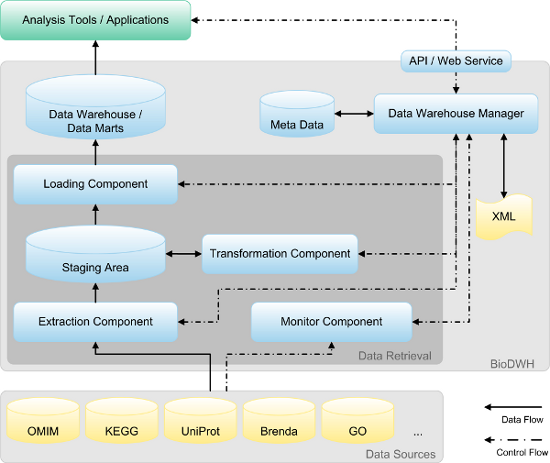
\includegraphics[width=4in]{figures/dwh_architecture.png}
\caption[BioDWH System Architecture.]{BioDWH System Architecture.
\label{fig:biodwh}}
\end{figure}

It is important to highlight the inclusion of a monitor system that keeps track on the need of updates from the different sources. Instead of direct access to the RDBMS, BioDWH provides an API that can be queried remotely, and a Graphical User Interface, that enables the configuration of the different components including monitors and parser besides the queuing and displaying of content.

Two projects have been reported in he literature to be using BioDWH: DAWIS-M.D. and VANESA. DAWIS-M.D. is oriented to metabolic data and integrates 11 different databases: BRENDA, EMBL, HPRD, KEGG, OMIM, SCOP, Transfac, Transpath, ENZYME, GO and UniProt. \cite{HIP2010}. VANESA uses DAWIS-M.D. in order to access important information for the modelling of biological processes and systems as biological networks\cite{BRI2014}.

\subsubsection{BioMart}
BioMart started by using the same principle of data warehousing that BioWarehouse, BioDWH and other projects of data warehouse in life science have follow: ``\emph{to create one universal software system for biological data management and empower biologists with the ability to create complex, customised datasets}'' \cite{KAS2011}.

With this object in mind BioMart have grown from an extension to the Ensembl website for data mining, to become an international effort for the integration of biological data. This has been achieve by first defining a general software infrastructure for further customisation, and then extending this architecture in order to support multi-database repositories as a data federation system, where all the entities use a predefined relational schema, that is generic enough to support any kind of data.

\begin{figure}  
\centering
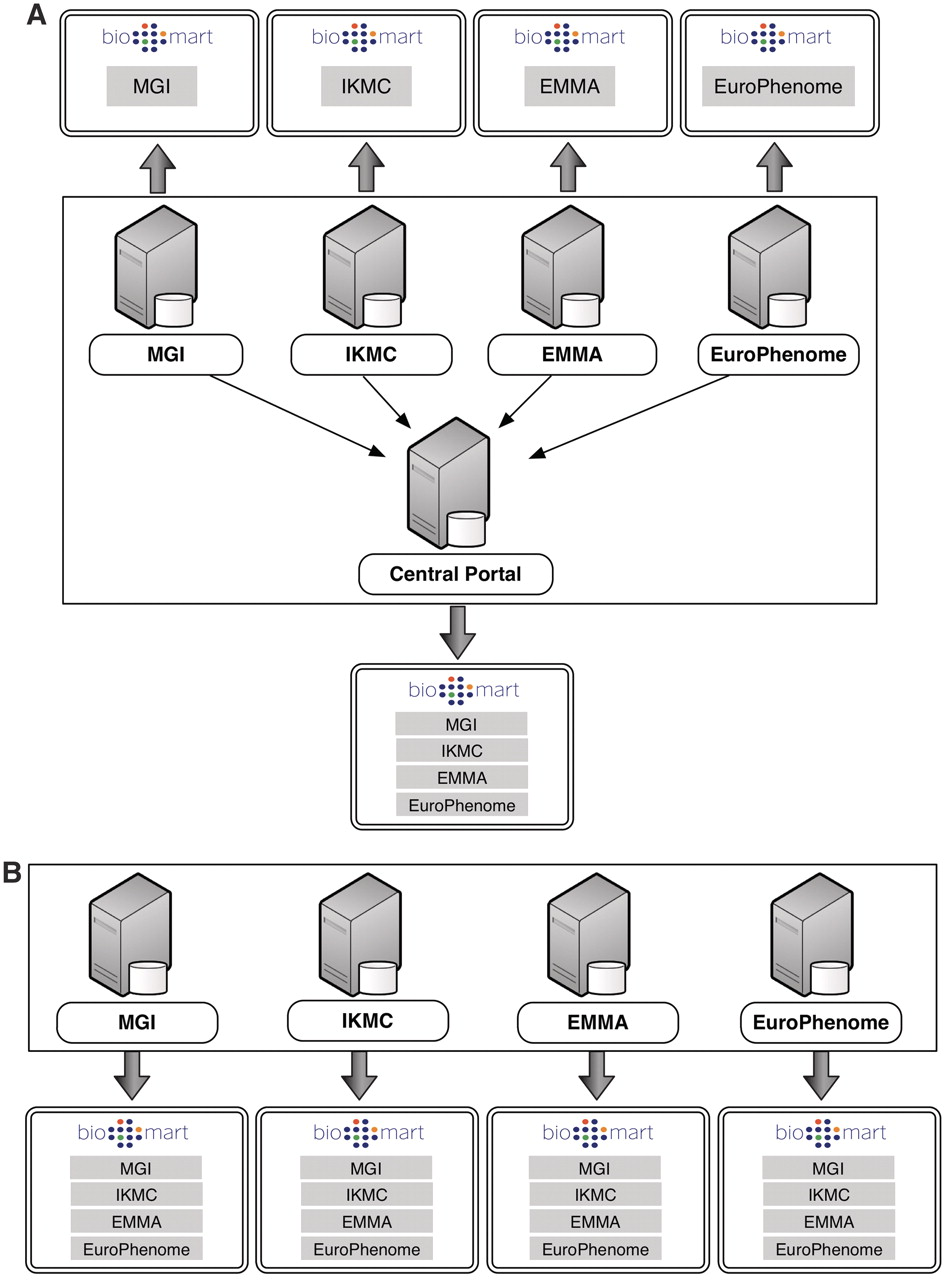
\includegraphics[width=\textwidth]{figures/biomart.png}
\caption[Biomart Portal Architecture.]{Biomart Portal Architecture. The portal can be set either with a master/slave or with a peer-to-peer configuration.
\label{fig:biomart}}
\end{figure}

Given the inclusion of a multi-database paradigm, the BioMart team developed a server that provide access to a collection of sources called a BioMart Portal. Figure \ref{fig:biomart} shows the 2 possible configurations of the BioMart Portal. In the configuration (a) each data source serves their own data and an independent server works as a central portal generating a unified view of the whole system. Alternatively, in the configuration (b) all the data source are treated as peers and they communicate with each other in order to be able to provide not only their own data, but also its peers' data.

BioMart includes a tool to automatically transform any 3rd form normalised database schema into the reverse-star scheme type used by this system. Once the dataset have been transformed, BioMart provides different view ports to it: Web-based Graphic Interface, Restful services and API connectors using Java.

\subsubsection{BioMOBY}
BioMoby is one the attempts to bring the promises of the semantic web into bioinformatics, proposing an architecture for the discovery and distribution of data though web services using multiple proposed standards of the World Wide Web Consortium (W3C) such as the Simple Object Access Protocol (SOAP). Its main goal is to provide access to biological data and services with a common format among the different sources \cite{WIL2002}.

The strategy of BioMoby is to have define a minimalistic entity to describe the data in such a way that different types of data can use the same schema.
This structure has been called the MOBY object, and is compose by 3 values: The MOBY object type (e,g. Sequence), a namespace identifier (e.g. Genbank/AC) and an accession number (e.g. AY070397.1). MOBy object types are defined using XML Schemas (XSD) reflecting a hierarchical relationship among them.

An important component go the BioMoby ecosystem is the MOBY Central: a server that contains information not only about available services, but also their association with MOBY objects for input and output. With this information a MOBI client can suggest paths to follow depending of the current type of your data. Moreover the intrinsic semantics of this approach is the ideal environment to create cohesive workflows.

\begin{figure}  
\centering
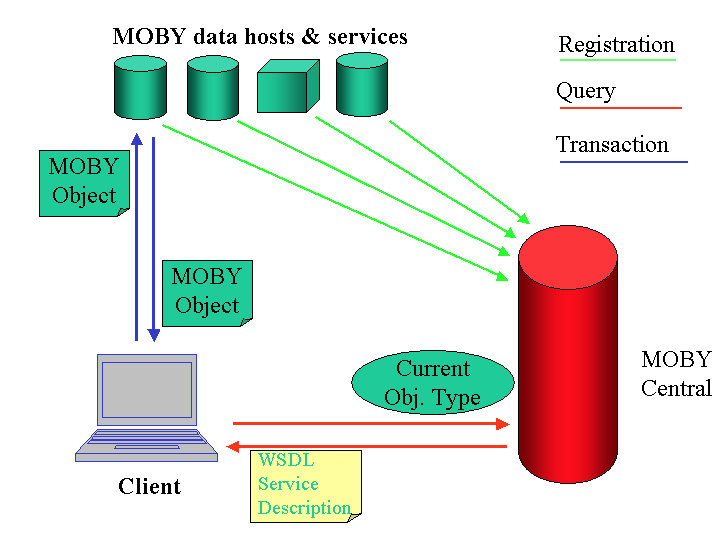
\includegraphics[width=4in]{figures/MOBY_Overview.png}
\caption[BioMoby Overview.]{BioMoby Overview.
\label{fig:biomoby}}
\end{figure}

Figure \ref{fig:biomoby} shows the adaptation done by BioMOBY to the classic web services architecture: Once all services have to register to the MOBY central, a client can query it to know which services can be used with the current MOBY Object. Besides the discovery feature, the central repository has the capability of generating a Web Service Description Language (WSDL) document that can be use in the corresponding service, where both in put and output are MOBY Objects.

A more recent iteration on the development of MOBY was described in \cite{VAN2009}: Moby-2. The objectives of the project have been extended and its focus on semantic web technologies is stronger, where the MOBY Central will take the form of a Resource Description Framework (RDF) triple store and will support the functionalities of a SPARQL endpoint. All this with the object of allowing semantic queries over multiple sources. The reported status of the project was a prototype, but promised to contribute towards a distributed, machine-readable semantic web of life science data.

\subsubsection{Bio2RDF}
A simplified view of the Semantic Web can be defined as a network where the nodes represent any entity that can receive a name and the edges correspond to the characteristics used to describe the relationships between the nodes. The RDF format is an XML-based language that describes this relationships as a set called ``triple'' that contains subject, predicate and object.

Bio2RDF uses RDF documents to be able to create a knowledge base that take advantage of existing developments on the semantic web to build a mashup of data in the bioinformatics domain.  \cite{BEL2008}.

One of the main objectives of Bio2RDF is to extract information from the most important bioinformatic databases, transform its content into RDF, and load it into a triplestore. It is within a triplestore than discovery of new knowledge happens through recombination analysis of the loaded data. In this sense Bio2RDF follows the approach of a data warehouse of semantic data.

As part of the project a set of software tools that convert different datasets into RDF called ``Rdfizers'' were created. There is one rdfizer for each source, however they can be grouped in 3 types depending on the origin of the data: XML to RDF, SQL to RDF, and text file to RDF. For big resources such as UniProt or PubMed were programmatic access to the data are provided, the rdfizer works on-demand, which means that only stores some of the data for cache purposes and the RDF files are created on the fly. Any other source gets copied into the centralised repository in order to offer quick responses.

The Bio2RDF approach can be summarised in three steps: (1) build a list of namespaces for data providers, (2) analyse a data source to represent it in an RDF model and (3) develop rdfizer to convert the information. The resulting dataset is sorted in the triplestore in order to connecting all together.

Bio2RDF used an extended version of Sesame as the triplestore and on its 2nd release was changed to Virtuoso in order to offer a better support to SPARQL, which is the most widely used query language for semantic web data. Other tools such as Protégé: an ontology editor, the Piggy Bank: a semantic browser for Firefox and Welkin: a RDF graph visualiser are use within Bio2RDF, all of them well known projects for the semantic web community.
 
 

\subsubsection{SADI}
The Semantic Automated Discovery and Integration (SADI) project has its roots in the learnings from BioMoby, particularly  Moby-2. however, unlike BioMoby, SADI is not a data typing system; the goals of SADI are centred in the proposal of patterns and best practices to use web services connected through semantic web technologies to enable the creation of interoperable and integrative bioinformatics software. \cite{WIL2011}.

The biggest change introduced by SADI in respect to SOAP web services is to replace the defined languages for communication between the web services parts (e.g. WSDL, XML Schema,UDDI) for structured versions of semantic web languages: RDF and the Ontology Web language (OWL). The authors go as far as to say that XML Schema is the problem causing the failure of most precedent interoperability architectures.

Here is is the description of an interaction with a SADI service: A client request the service description via HTTP GET, and the server responds with a document containing references to OWL classes describing input and output datatypes for the service; The client uses data formatted in RDF that follows the received description to submit an HTTP POST request, which is captured by the server, that in turn uses it to execute the service and generate a response in RDF format.

The adoption of HTTP methods for communication follows the positive reception of ``RESTful'' Architectures. SADI does't claim to follow a RESTful architecture, but it sees the potential of it and uses some of its principles, this is partially a response of the general sense of dislike of the SOAP architecture around the bioinformatics community.

The use of a good ontology to connect services is seen in SADI as the key component to meaningful interoperability, where the interaction between servers is guided by biological knowledge and not only by technicalities such as format and availability.

As part of the project, software components have been developed in order to facilitate the adoption of the recommendations including plugins for Taverna and Protege, and a  prototype of all the components (i.e. Servers and clients) is available at http://biordf.net/cardioSHARE/
%it uses the My Grid/Moby service ontology when defining the services, but the authors claim that this can be change in case a more suitable ontology is developed in the future.

\subsubsection{BioPAX}
The Biological PAthway eXchange (BioPAX ) is a community driven effort to develop a standard language to facilitate knowledge representation of biological pathways at molecular and celular level in order to enable the systematic collection, distribution and integration of pathway data from heterogeneous sources \cite{DEM2010}.

BioPAX also takes input from the semantic web community. In this case OWL is used to define an ontology to describe pathways information, that can be use to interconnect the multiple resources on this domain. BioPax has among others, been used to describe (1) metabolic pathways following the abstraction: ``enzyme, substrate, product''; (2) signalling pathways for biochemical reactions, binding, and catalysis events; (3) gene regulatory networks involving transcription aand translation events and its control; (4) protein protein interaction and protein-DNA interactions; and (5) genetic interactions i.e. when the phenotype of perturbing 2 genes is different than the expected known of the perturbation of each isolated gene.

The BioPAX ontology is the result of ongoing periodical workshops that involves the different stakeholders on the biological pathways field. Incremental versions of the agreement, also called levels have been developed with the concept that newer levels can replace older ones, currently the higher one is level 3.

A tool set called Paxtools has been developed as part of the project. The main features of this software include an implementation of the specification as a software model, the support of OWL properties, asyndetic validator, transformation scripts between levels, import and export to other formats. Reasons why Paxtools can and have been used as the framework to develop other tools.


\subsubsection{The HUPO Proteomics Standards Initiative}
The Proteomics Standards Initiative (PSI) collaborative initiative run by volunteers and coordinated as a work group of the HUman Proteome Organisation (HUPO) which object is to define standards  to enable capture, comparison, exchange and verification of proteomics data. \cite{HER2006}. PSI is the result of a common effort from the interested parts on the proteomics domain.

This effort can be categorised in three major infrastructure elements: (1) An specification of the Minimum Information About a Proteomics Experiment (MIAPE), (2) data exchange formats that are complaint with MIAPE, and (3) the use of controlled vocabularies (CV) in order to ensure the consistency on the data content. In this way the proposed standard can be stable while its content can evolve by updating the CV.

These recommendations are not intending to specify the methods and procedures for proteomics experiments, and should be seen as reporting guidelines.

This initiative has been growing for the last 10 years, and now its standards are widely adopted in the proteomics community. The proposed specifications cover different branches of the field, for instance the PSI-MI formats were defined to deal with Molecular interactions data, PSI-MS works on standards for mass spectrometry data and PSI-MOD focuses on protein modifications.

However even if all the parts follow the recommendations, an strategy to integrate this data is required, it is for the reason that he PSI common query interface (PSICQUIC) was created: a community standard that enables programatic access to molecular-interaction data resources \cite{ARA2011}. This proposal includes a query language (MIQL) and an architecture to execute a query on distributed sources.

Figure \ref{fig:psicquic} shows the architecture of PSICQUIC. The idea is that several samples from an organism can be processed by different experiments and its findings can be published in independent articles, which consequently can be stored in more than one interaction database. PSICQUIC proposes that the providers support an extra layer to access this information, which can be queried using MIQL and with responses follow the PSI-MI formats; in this way a client can use a single query over multiple resources and bring a unified image.


\begin{figure}  
\centering
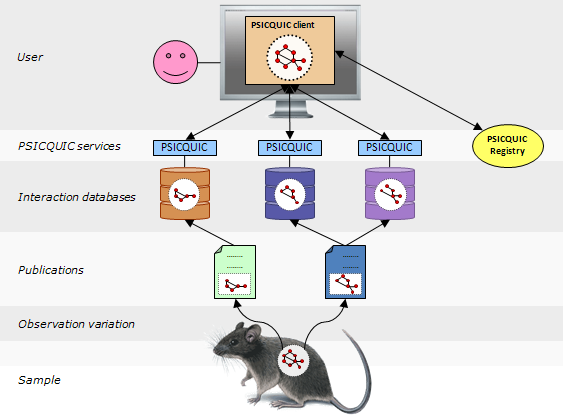
\includegraphics[width=4.3in]{figures/psicquic.png}
\caption[PSICQUIC Architecture.]{PSICQUIC Architecture.
\label{fig:psicquic}}
\end{figure}

The PSI group recognises the importance in providing software tools to impulse the adoption of the proposed standards. The most recent implementation of the PSICQUIC web service was released when the version 1.3 of the PSICQUIC specification was made public in 2013 \cite{DEL2013}. The providers of molecular interaction data are now asked to implement a number of methods in order to support both SOAP and REST web services. 

The Web service methods will generally accept a MIQL query as input and generate an output in either PSI-XML or PSI-MITAB in one of its most recent versions. This implementation is based on the Apache Solr indexing software (http://lucene.apache.org/solr/), this is reflected on the constitution of MIQL, which is an extension of the Lucene Query language used in Solr. This implementation is freely available for any provider that desire to share its data to the PSI community.

Besides the server, PSICQUIC also provides client libraries to facilitate the access to the information from different programming languages: Java, Perl, Python. There are ready to use clients, for example the PSICQUIC View accessible from http://www.ebi.ac.uk/Tools/webservices/psicquic/view/main.xhtml or plugins for Cityscape and the R Bioconductor package.

The last component of the PSICQUIC architecture is the registry, in which information about the available providers is stored as tags. This metadata can be used to query the registry as a RESTful service in order to facilitate the discovery of molecular-interaction data providers.

\subsubsection{Taverna}
Taverna was originally conceived as a tool for not experts programmers to design, execute and share workflows of web services \cite{HUL2006}. Bioinformatics web services can be a way of providing the available data in a data source (e.g. the PSI services), but most traditionally web services are seen as a remote software component that receives some input data, processes it and generates output data; leaving most of the processing load to the service provider, allowing small groups to run high throughput analysis.

Taverna is a tool that allows to create ``recipes'' of combined web services or already composed workflows to execute a higher level computational experiment. The Taverna workbench is a graphical interface that allows the design of workflow, that can be execute it either on the same workbench or in independent runner tools such as the Taverna command-line application, the Taverna server or the Taverna lite installation.

By 2013 the Taverna project reported to have access to over 8000 service operations \cite{WOL2013}, with such a big number of resources, there is a necessity on make them searchable; this is the goal of the BioCatalogue: a registry for web services were both REST and SOAP services can be discover using their metadata. Taverna supports the search on the BioCatalogue and inclusion of a chosen web service through its workbench tool.

It is often necessary to do intermediate processing to be able to connect two services, where for example one produces the data that is required for the second but in a different format. Taverna provide a set of what they call ``shim'' services to supply this need. Other type of services that are supported by Taverna are local, grid and cloud services, access to BioMart, R-Scripts and distributed command-line scripts.

The number of ready-to-use workflows have grown in recent years, that is great for researchers that need an start point for their experiment, how ever this number is so big that finding the right pipeline for an  analysis was not an easy task, for this reason MyExperiment was developed, it not only support Taverna workflows but also other systems such as Galaxy (discussed below). To run a workflow found in the MyExperiment repository in Taverna, is as easy as to copy the URL into the workbench importer, adjust the parameters and pressing ``run''.


\subsubsection{Galaxy}


\subsubsection{WikiGenes and WikiProteins}

\subsection{The Distributed Annotation System}
The Distributed Annotation System (DAS) is... \cite{JEN2008} and I can use Fig.~\ref{fig:das}. to explain:
\begin{figure}  
\centering
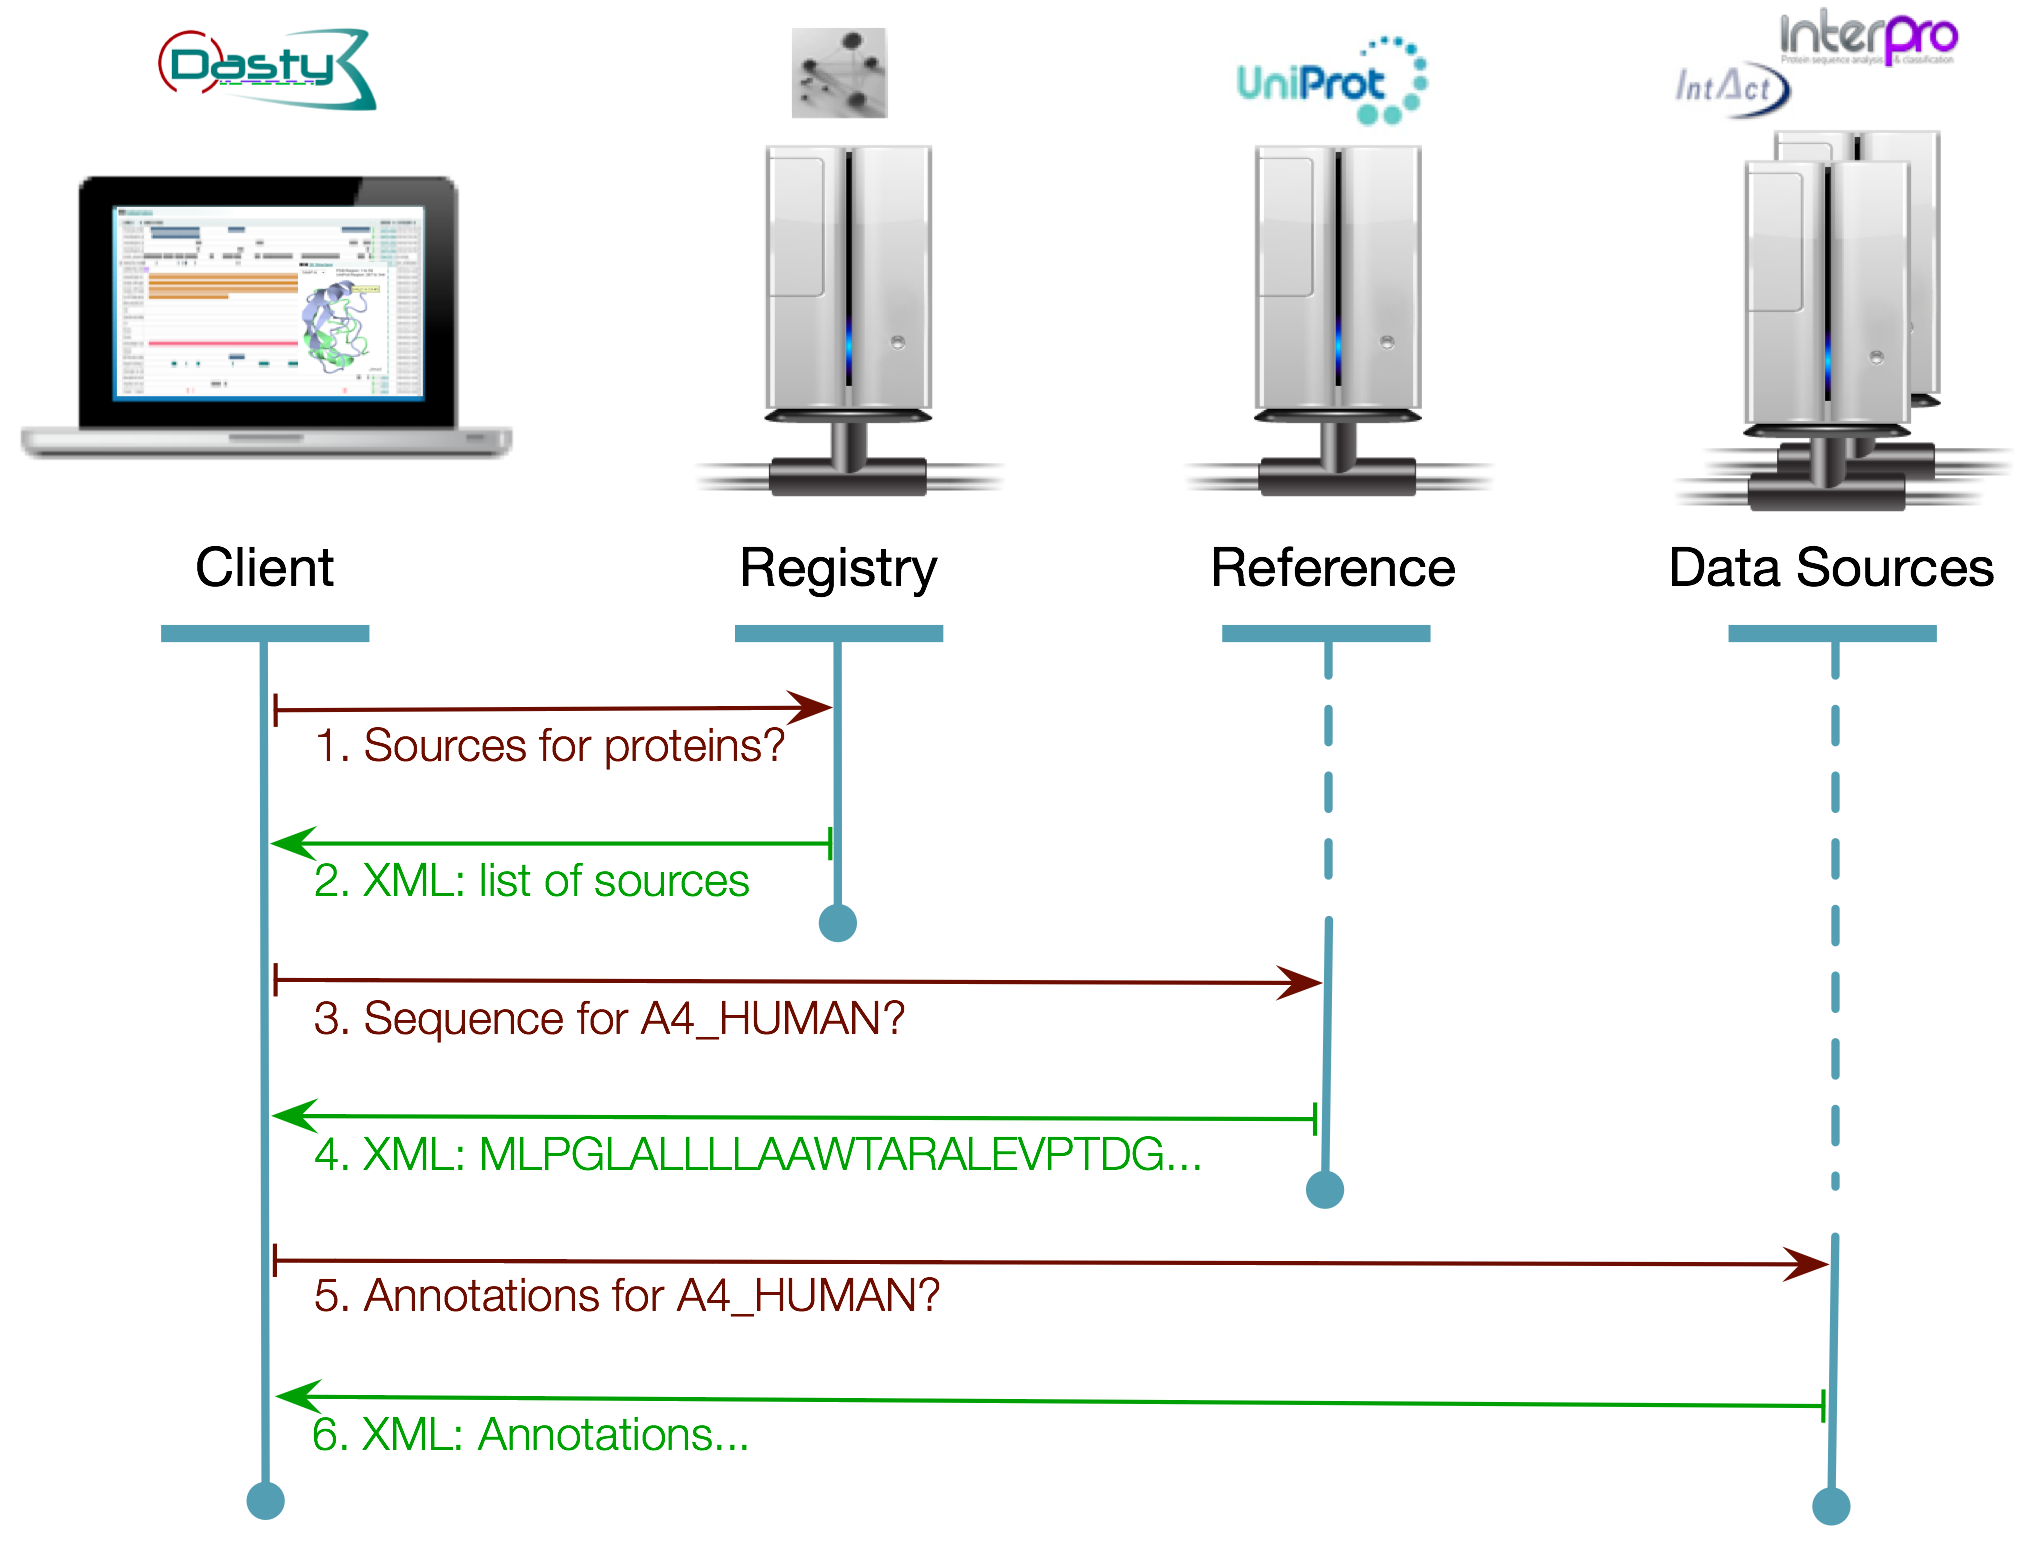
\includegraphics[width=\textwidth]{figures/DAS.png}
\caption[DAS Flow of Information.]{Flow of information in a standard query in the Distributed Annotating System.
\label{fig:das}}
\end{figure}
we should describe Dasty3 \cite{VIL2011}


\subsection{Discussion}
Besides the primary data coming from \emph{in-vitro} experiments, there are hundreds of sources consolidating data that results from \emph{in-silico} analysis.

\begin{savequote}[75mm] 
Our posturings, our imagined self-importance, the delusion that we have some privileged position in the Universe, are challenged by this point of pale light.
\qauthor{Carl Sagan, Pale Blue Dot, 1994} 
\end{savequote}
\section{Visualization}
The field of visualization aims to represent data in a way that non evident features became visible. The developed techniques in this search varies from simple ones (e.g. histograms) to very elaborated (e.g. environments just visible using 3D virtual reality rooms).

The uses of visualization techniques are as diverse as fields are in the world, from weather forecast in the news to the analysis of the captured data in the Large Hadron Collider. In the field of our interest: bioinformatics, the use of visualization methods is also abundant and sub-fields such as genomics, proteomics, population variance, etc. have plenty of examples were different techniques have been implemented with the purpose of making sense of biological data via visual representations.

The section below is a review of the most relevant existing tools in different bioinformatics fields.
\subsection{Visualization tools in Bioinformatics}
Small intro for the subsection
\subsubsection{Genomics}
Ensembl, mykarioView, Dalliance, IGV, Tablet, BAMView
\subsubsection{Proteomics}
Dasty, Interpro
\subsubsection{Protein Interaction}
\subsubsection{Population Variation}
\subsubsection{General Research}
To talk about statistical graphs and things like heat maps, phylogenetic trees, etc.


\section{Thesis outline}
